

\section{Theoretical Justification of the Robustness Properties of Bayesian Learning}
\centering
\frame{Theoretical Justification of the Robustness Properties of Bayesian Learning}

\begin{frame}{Robustness of Bayesian Learning under System Parameter Uncertainties}
  \textcolor{green}{Proof of concept}:
  Compare the performance of deterministic and stochastic optimal control
  \begin{small}
      \begin{columns}
        \begin{column}[t]{0.48\linewidth}
          \begin{exampleblock}{Deterministic}
              \begin{equation*}
                  \begin{aligned}
                  \underset{\theta }{\text{min}} 
                  &\quad \mathcal{J} = \int_0^T \left(\frac{1}{2}qx(t)^2 + \frac{1}{2}ru(t)^2 \right) dt \\
                  \text{subject to} 
                  &\quad \dot{x} = \hat{p}x + u,\\
                  &\quad u(x) = \theta x. \\ 
                  \end{aligned}    
              \end{equation*}
  \end{exampleblock}
\end{column}
% \pause
\begin{column}[t]{0.49\linewidth}
  \begin{alertblock}{Stochastic}
      \begin{equation*}
          \begin{aligned}
          \underset{f(\theta)}{\text{min}} 
          &\quad \mathcal{J} = \int_0^T \left(\frac{1}{2}qx(t)^2 + \frac{1}{2}ru(t)^2 \right) dt \\
          \text{subject to} 
          &\quad \dot{x} = px + u,\\
          &\quad u(x) = \theta x, \\ 
          &\quad \theta \sim f(\theta), \\ 
          &\quad p \sim \mathcal{N}(\hat{p}, \sigma_p^2).  
          \end{aligned}    
      \end{equation*}
  \end{alertblock}
\end{column}
\end{columns}
\end{small}

\end{frame}

\begin{frame}{}
  \begin{align*}
    x(t) &= e^{(p + \theta)t}, \;\; x(0) = 1, \\
    u(x) &= \theta x.
  \end{align*}
  \begin{columns}[T]
    \begin{column}{0.49\linewidth}
      Deterministic policy
      \begin{align*} 
        \mc{J} &= \int_0^T \left(\frac{1}{2}qx^2 + \frac{1}{2}ru^2 \right) dt,\\
        \mc{J}_\infty &= -\frac{1}{4}\frac{q+r\theta^2}{\hat{p}+\theta}, \\
        \nabla_\theta \mc{J}_\infty &= -\frac{r}{4}\frac{(\hat{p}+\theta)^2 - \left(\hat{p}^2
        + \nicefrac{q}{r}\right)}{(\hat{p}+\theta)^2} = 0, \\
        \theta^\star &= -\hat{p} - \sqrt{\hat{p}^2 + \nicefrac{q}{r}}.
      \end{align*}
    \end{column}
    \begin{column}{.01\textwidth}
      \rule{.1mm}{.6\textheight}
    \end{column}
    \begin{column}{0.46\linewidth}
      Stochastic policy
      \begin{align*}
        g(p) &:= -p - \sqrt{p^2 + \nicefrac{q}{r}}, \\
        f_{\theta^\star}(\theta^\star) &= f_p\left(g^{-1}(\theta^\star)\right)
        \abs{\frac{d}{d\theta}g^{-1}(\theta^\star)}. 
      \end{align*}
    \end{column}
  \end{columns}
\end{frame}

\begin{frame}
  \begin{figure}
      \includegraphics<1>[width=0.7\linewidth]{optimal-dist_1.eps}
      \includegraphics<2>[width=0.7\linewidth]{optimal-dist_2.eps}
      \includegraphics<3>[width=0.7\linewidth]{optimal-dist_3.eps}
  \end{figure}
  \begin{itemize}
      \only<1,2,3>{\item $\hat{p} = 5, \sigma_p = 5$}
      \only<1,2>{\item The stochastic solution gives an exponential distribution over optimal
      $\theta$.}
      \only<2>{\item Red shows deterministic solution.}
      \only<3>{\item The deterministic solution is completely unaware of the effects of uncertainties.
        For e.g., the true dynamics may be unstable under $\theta^\star$. The
        stochastic controller reasons about stability for various parameters.  
      }
  \end{itemize}
  \vspace{2cm}
\end{frame}

\begin{frame}{Robustness Under System Parameter and Measurement Uncertainties}
  \begin{small}
    \begin{exampleblock}{Stochastic optimal control}
        \begin{equation*}
          \begin{aligned}
            \underset{f(\theta)}{\text{min}} 
            &\quad \mathcal{J} = \int_0^T \left(\frac{1}{2}qx(t)^2 + \frac{1}{2}ru(t)^2 \right) dt \\
            \text{subject to} 
            &\quad \dd x = (p+\theta)x(t) \dd t + \theta\sigma \dd W_t,\\
            &\quad \hspace{0.7cm} \theta \sim f(\theta), \\ 
            &\quad \hspace{0.7cm} p \sim \mathcal{N}(\hat{p}, \sigma_p^2).  
            \end{aligned}       
        \end{equation*}
  \end{exampleblock}
\end{small}
\hspace{-3.0cm}where $W_t$ is the Wiener process, $\sigma$ is the standard deviation of the
noise. 
\begin{itemize}
  \item With $x(0) = 1$, the solution to the SDE is 
  \begin{align*}
    x(t) &= e^{(p+\theta)t} + \theta\sigma \int_0^t e^{(p+\theta)(t-s)}dW_s.
  \end{align*}
  \item We can compute the expected cost numerically as 
  \begin{align*}
    \mathbb{E}[\mathcal{J}] &= \mathbb{E}_p[\mathbb{E}_W[\mathcal{J} \mid p]].
  \end{align*}
\end{itemize}
\end{frame}

\begin{frame}{}

  \begin{columns}

    \begin{column}[t]{0.48\linewidth}
      \begin{figure}
        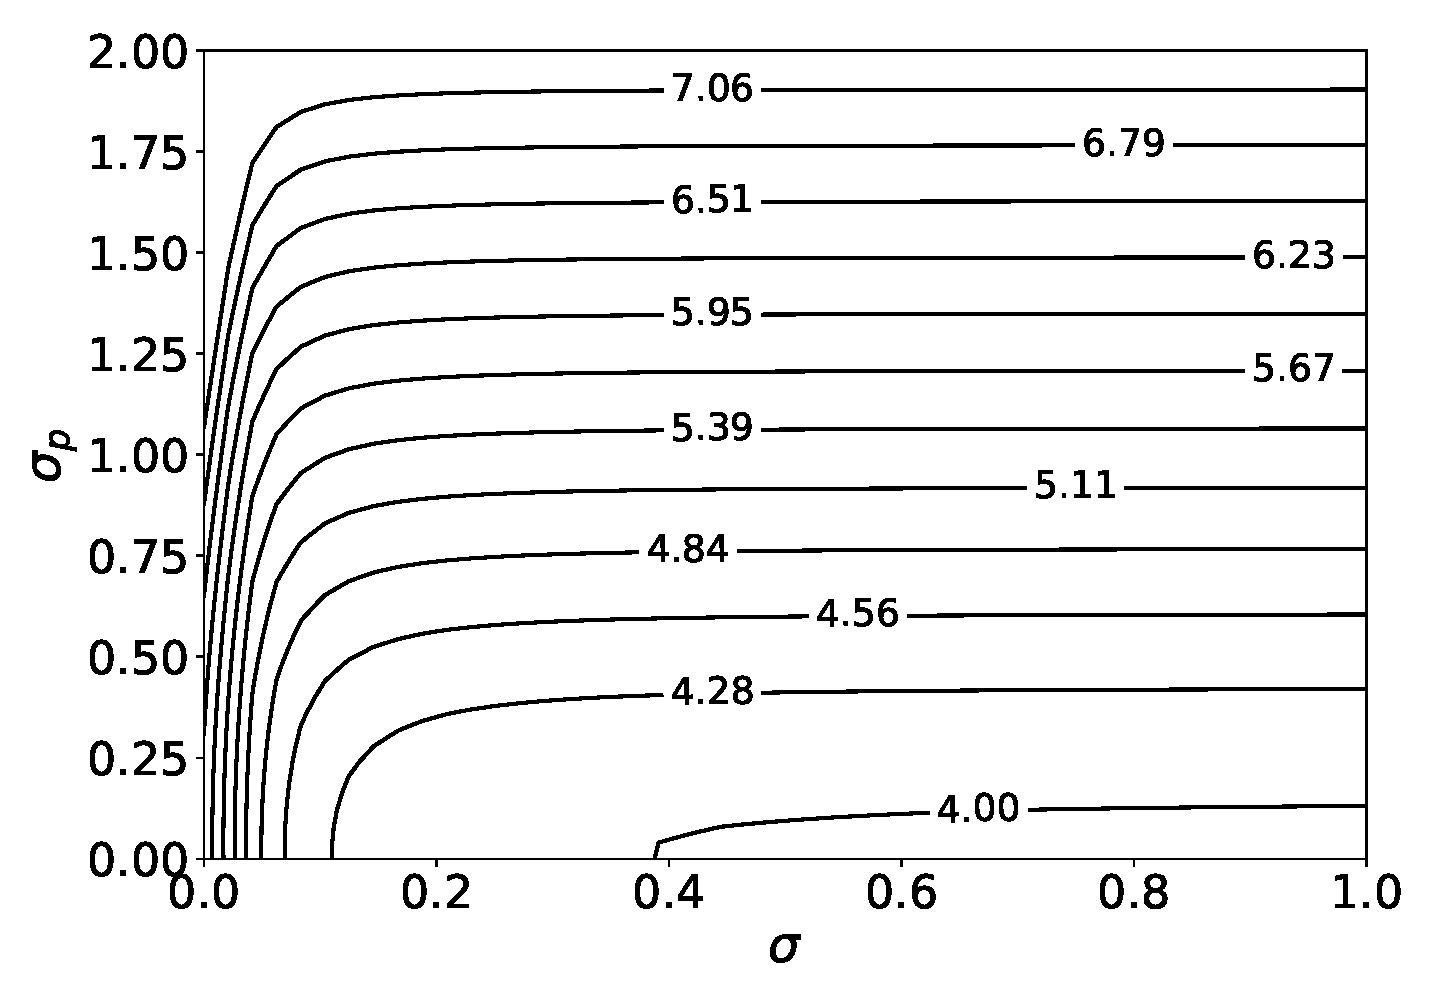
\includegraphics[width=0.9\linewidth]{optimal_ctrl.eps}
        \caption{The optimal controller parameter magnitude $|\theta^\star|$ that minimizes $\mathbb{E}[\mathcal{J}]$}
      \end{figure}
    \end{column}

    \begin{column}[t]{0.46\linewidth}
      \begin{figure}
        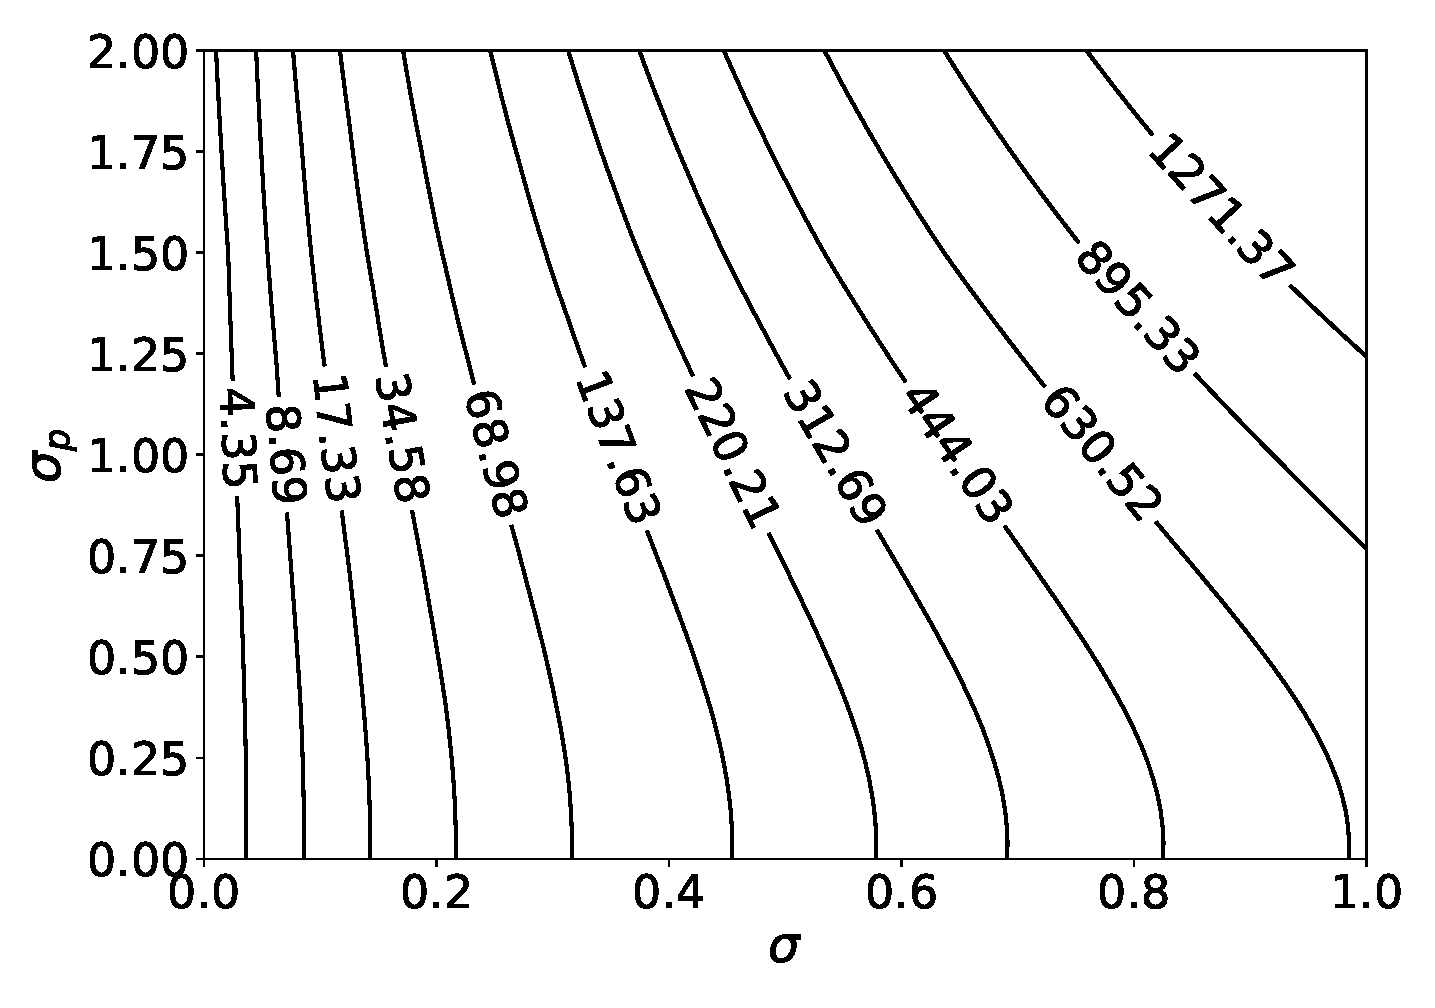
\includegraphics[width=0.9\linewidth]{optimal_cost.eps}
        \caption{The minimal expected cost $\mathbb{E}[\mathcal{J}]$}
      \end{figure}
    \end{column}

  \end{columns}

\end{frame}

\begin{frame}{Discussion}
  % \begin{itemize}
  %   \item The discrepancy between the stability of the deterministic parameter
  %   $\theta^\star$ and the expected control parameter $\mathbb{E}(\theta^\star)$
  %   shows that the deterministic policy is overconfident.
  %   \item The expected cost $\mathbb{E}[\mathcal{J}]$ increases considerably
  %   with measurement error.
  % \end{itemize}
  % \hspace{-12cm} \textbf{Conclusions}
  \begin{itemize}
    % \item It is best to find a controller that works best on average. Otherwise,
    % we are naively hoping for the actual system parameters to be very close to
    % the nominal one and the measurement noise is zero.
    \item It is more robust to develop a stochastic controller given system
    parameter uncertainties and measurement noise.
    \item We employ Bayesian learning to design a stochastic policy from
    data-driven techniques.
  \end{itemize}
\end{frame}

\section{Background: Bayesian Learning}
\frame{Background: Bayesian Learning}


\begin{frame}[c]{Bayesian Learning}
  \begin{itemize}
  \item \textcolor{green}{Objective} : Learn a target function $F(x; \theta) :
  \mathcal{X} \rightarrow \mathbb{R}^t$ that best parameterizes the source of a
  dataset $\mathcal{D}$ with inherent noise.
  \item The target function is parameterized by the random variable $\theta$.
  \item The task is to learn the distribution of $\theta$ given prior belief.
  \begin{equation*}
    p(\theta | \mathcal{D}) = \frac{ \overbrace{p(\mathcal{D} \mid \theta)}^{\textcolor{blue}{likelihood}} \overbrace{p(\theta)}^{\textcolor{green}{prior}}}{\underbrace{\int_\theta p(\mathcal{D} \mid \theta') p(\theta') d\theta'}_{\textcolor{red}{evidence}}}
  \end{equation*}
    \item The evidence is intractable in most cases.
    \item There are techniques used to find the exact or an approximate posterior.
  \end{itemize}
\end{frame}

\begin{frame}{Bayesian Learning}
  \frametitle{Posterior Distribution: Variational Inference}
  \begin{itemize}
    \item \textcolor{green}{Variational inference}: select a distribution $q(\theta;z)$
    and adjust the distribution parameters $z$ to best fit to $p(\theta \mid \mathcal{D})$.
    \item The objective is to learn the distribution parameters $z$, such that
    the Kullback-Leibler (KL) divergence given by
    \begin{align*}
      D_{KL} &= \mathbb{E}_{\theta \sim q}\left [ \log \frac{q(\theta;z)}{p(\theta \mid \mathcal{D})} \right] \\
      &= \log(p({\mathcal{D})}) - \mathbb{E}_{\theta \sim q} \left[ \log \frac{ p(\mathcal{D} \mid \theta)p(\theta;z)}{q(\theta;z)}\right]
    \end{align*}
    is minimized.
    \item This is similar to maximizing the \textit{evidence lower bound} (\textsc{Elbo}):
    \begin{align*}
        \mathcal{L}(\mathcal{D},z) = \mathbb{E}_{\theta \sim q} \left[\log( p(\mathcal{D} \mid \theta)p(\theta;z)) - \log(q(\theta;z)) \right]
    \end{align*}
  \end{itemize}
\end{frame}

% \begin{frame}{Bayesian Learning}
%   \frametitle{Posterior Distribution: Variational Inference}
%   \begin{itemize}
%     \item \textcolor{green}{Variational inference}: given the form of the
%     likelihood and the prior distributions, the posterior distribution $q(\theta;z)$
%     is chosen from the conjugate family.
%     \item The objective is to learn the distribution parameters $z$, such that
%     the \textit{evidence lower bound} (\textsc{Elbo}) given by
%     \begin{align*}
%         \mathcal{L}(J,z) = \mathbb{E}_{\theta \sim q} \left[\log( p(J \mid \theta;z)p(\theta;z)) - \log(q(\theta;z)) \right]
%     \end{align*}
%     is maximized.
%   \end{itemize}
  
    % \begin{equation*}
    %     \begin{aligned}
    %       \underset{z}{\text{maximize}} 
    %       &&\quad \mathcal{L}(J,z) &= \mathbb{E}_{\theta \sim q} \left[\log p(J \mid \theta;z)p(\theta;z) - \log(q(\theta;z)) \right] \\
    %       \text{subject to} 
    %       &&\quad M_d^\theta &= \big( M_d^\theta \big)^\top \succ 0, \\
    %       &&\quad J_2^\theta &= -\big( J_2^\theta \big)^\top, \\
    %       % &&\quad q^\star &= \underset{q}{\textrm{argmin}} \; V_d^\theta.  \\
    %       &&\quad q^\star &= \underset{q}{\text{argmin}}\; V_d^\theta,
    %     \end{aligned}    
    %     % \label{eq:finite_optim}%
    %   \end{equation*}
      % where $p(\theta;z)$ is the prior distribution and the likelihood is $p(J
      % \mid \theta;z) = \mathcal{N}\left(0, s\right)$ for chosen standard
      % deviation $s$.
% \end{frame}
